\documentclass[12pt]{standalone}

\usepackage{tikz}
\usetikzlibrary{arrows}

\begin{document}

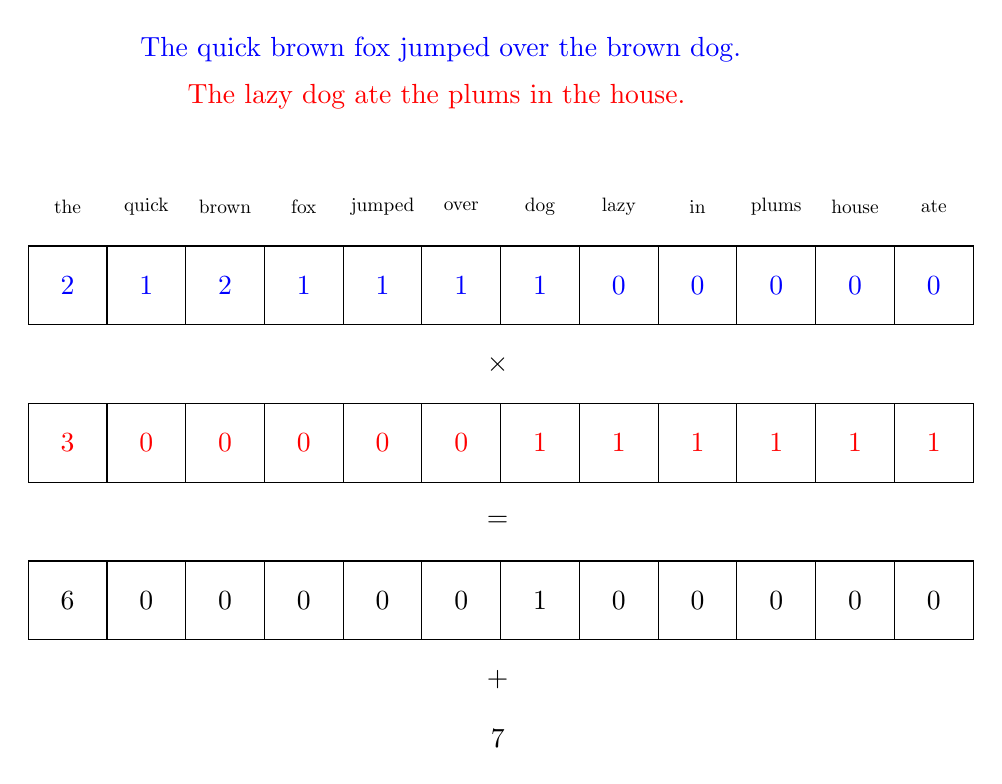
\begin{tikzpicture}

\tikzstyle{count} = [rectangle, minimum size=1cm, draw=black]
\tikzstyle{blue} = [text=blue]
\tikzstyle{red} = [text=red]
\tikzstyle{word} = [scale=0.7]
\tikzstyle{doc} = [anchor=west]
\tikzstyle{ellipsis} = []

\node[doc,color=blue] at (0.8, 3.0) {The quick brown fox jumped over the brown dog.};
\node[doc,color=red] at (1.4, 2.4) {The lazy dog ate the plums in the house.};

\node[word] at (0, 1) {the};
\node[word] at (1, 1) {quick};
\node[word] at (2, 1) {brown};
\node[word] at (3, 1) {fox};
\node[word] at (4, 1) {jumped};
\node[word] at (5, 1) {over};
\node[word] at (6, 1) {dog};
\node[word] at (7, 1) {lazy};
\node[word] at (8, 1) {in};
\node[word] at (9, 1) {plums};
\node[word] at (10, 1) {house};
\node[word] at (11, 1) {ate};

\node[count, blue] at (0, 0) {2};
\node[count, blue] at (1, 0) {1};
\node[count, blue] at (2, 0) {2};
\node[count, blue] at (3, 0) {1};
\node[count, blue] at (4, 0) {1};
\node[count, blue] at (5, 0) {1};
\node[count, blue] at (6, 0) {1};
\node[count, blue] at (7, 0) {0};
\node[count, blue] at (8, 0) {0};
\node[count, blue] at (9, 0) {0};
\node[count, blue] at (10, 0) {0};
\node[count, blue] at (11, 0) {0};

\node[doc] at (5.2, -1) {$\times$};

\node[count, red] at (0, -2) {3};
\node[count, red] at (1, -2) {0};
\node[count, red] at (2, -2) {0};
\node[count, red] at (3, -2) {0};
\node[count, red] at (4, -2) {0};
\node[count, red] at (5, -2) {0};
\node[count, red] at (6, -2) {1};
\node[count, red] at (7, -2) {1};
\node[count, red] at (8, -2) {1};
\node[count, red] at (9, -2) {1};
\node[count, red] at (10, -2) {1};
\node[count, red] at (11, -2) {1};

\node[doc] at (5.2, -3) {$=$};

\node[count] at (0, -4) {6};
\node[count] at (1, -4) {0};
\node[count] at (2, -4) {0};
\node[count] at (3, -4) {0};
\node[count] at (4, -4) {0};
\node[count] at (5, -4) {0};
\node[count] at (6, -4) {1};
\node[count] at (7, -4) {0};
\node[count] at (8, -4) {0};
\node[count] at (9, -4) {0};
\node[count] at (10, -4) {0};
\node[count] at (11, -4) {0};

\node[doc] at (5.2, -5) {$+$};

\node[doc] at (5.25, -5.75) {$7$};

\end{tikzpicture}

\end{document}
